\chapter{Asking Women Billionaires How They Got Rich!}

This lecture is built out of reversals. It opens by spending surprise first and explanation later: a yacht, an oil-industry answer, a 2023 sale, a roughly \(\$90\) million equity figure, and the word ``billionaire.'' Only after that bait does the episode tell us what belongs to which case and why the numbers matter. Because no validated mathematical screenshots survived review for this lecture, the equations and figures below are transcript-led reconstructions. The aim is therefore not to imitate a board that never appears, but to preserve the lecture's actual rhythm: object first, mechanism next, and only then a more durable lesson about money, ownership, and strategy.

\section{Cold Open: Female Billionaires, Miami, and the Teaser Logic}

We should begin by not over-reading the opening. The teaser is a collage, not a single stable interview. Oil belongs to one later case, the \(\$90\) million equity figure belongs to another, and the yacht-side billionaire appears later still. The lecture uses this splice deliberately. It wants to prove access and scale before it explains method.

The true opening comes with the reset. The host names a global count,
\begin{equation}
N_{\text{female billionaires}} > 360,
\end{equation}
and then turns Miami into a field site. The city is not important for its weather or scenery. It matters because visible wealth is dense there, and the lecture wants to question that wealth at close range rather than admire it from a distance.

The governing move is simple. We begin with what can be seen and then refuse to stop there. A yacht, a Bentley, a G-Wagon, a marina, a valet line: all of these are only surfaces. The lecture keeps asking for the machinery underneath them.

\begin{figure}[h]
\centering
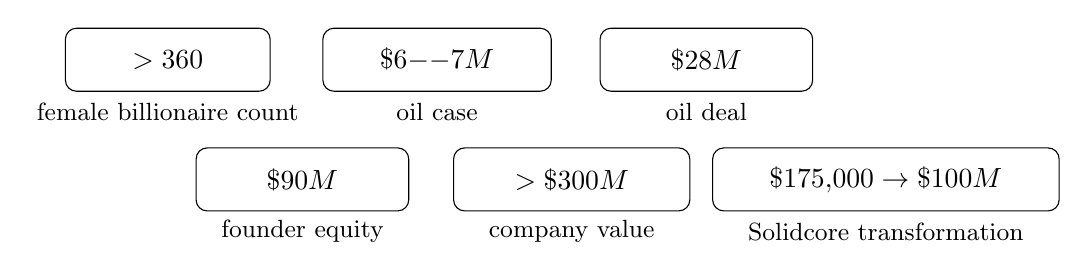
\begin{tikzpicture}[scale=0.95]
\node[draw, rounded corners, minimum width=2.6cm, minimum height=0.8cm] at (0,1.6) {\(>360\)};
\node[draw, rounded corners, minimum width=2.9cm, minimum height=0.8cm] at (3.6,1.6) {\(\$6\text{--}7\text{M}\)};
\node[draw, rounded corners, minimum width=2.7cm, minimum height=0.8cm] at (7.2,1.6) {\(\$28\text{M}\)};
\node[draw, rounded corners, minimum width=2.7cm, minimum height=0.8cm] at (1.8,0) {\(\$90\text{M}\)};
\node[draw, rounded corners, minimum width=3.0cm, minimum height=0.8cm] at (5.4,0) {\(>\$300\text{M}\)};
\node[draw, rounded corners, minimum width=4.4cm, minimum height=0.8cm] at (9.6,0) {\(\$175{,}000 \to \$100\text{M}\)};

\node at (0,0.9) {\small female billionaire count};
\node at (3.6,0.9) {\small oil case};
\node at (7.2,0.9) {\small oil deal};

\node at (1.8,-0.7) {\small founder equity};
\node at (5.4,-0.7) {\small company value};
\node at (9.6,-0.7) {\small Solidcore transformation};
\end{tikzpicture}
\caption{Transcript-based quantity strip for the lecture's opening logic. The cold open spends scale and surprise first, then later assigns each number to its proper case.}
\end{figure}

\section{Oil, Rule-Breaking, and the First Mechanics of Wealth}

The first full case is the woman stepping out of the G-Wagon. The lecture narrows quickly from object to industry. She is in oil. She has been a business owner for about sixteen years. The best one-year number she gives, explicitly softened by the host toward business revenue rather than personal income, is on the order of six to seven million dollars:
\begin{equation}
t_{\text{oil}} \approx 16\ \text{years},
\qquad
Y_{\text{oil}} \approx \$6\text{--}7\,\text{million}.
\end{equation}

\paragraph{Anecdote.}
The first principle she offers is not technical but social: well-behaved women rarely make history. Women who only play by the rules, she says, do not get very far.

\paragraph{Claim.}
In the lecture's sequence, this is not motivational garnish. It is a theory of entry. Exceptional commercial outcomes often require stepping where conventional permission structures would have made us pause.

\paragraph{Mechanism.}
The host immediately tests whether the doctrine leads anywhere concrete. What business made the most money? She answers: manufacturing solar panels and pumping crude oil. What was the biggest deal? First the number appears as about \(\$20\) million, then sharpens to the more stable figure,
\begin{equation}
D_{\text{max,oil}} \approx \$28\,\text{million}.
\end{equation}
The earlier number is best kept as conversational refinement rather than as a second settled datum. She then adds a detail that matters for tone: it was not formally her deal, but she closed it, in the oil business, at age twenty-one, and the commission was heavy.

The lecture is doing something precise here. It will not let the rule-breaking maxim float free. It places it next to years in business, next to sector-specific activity, and next to deal size. That is the first real pedagogical turn: attitude must cash out as operation.

The host keeps narrowing. Is she a buyer or seller? Both, depending on the market, she says, but above all a seller. And now a new piece of the mechanism appears. Her confidence in sales is rooted not only in bravado but in experience with people. She has sold for years, and she has done corporate customer service for years. In other words, persuasion and people-handling are treated as adjacent capacities, not separate ones.

\subsection{Question \& Answer}

\paragraph{Question.}
How does boldness become business method rather than just attitude?

\paragraph{Answer.}
The lecture answers by refusing to stop at the slogan. Boldness becomes method only when it attaches itself to a market, a sale, and a number. Here the sequence is exact: oil, sixteen years, six to seven million in a year, then solar panels and crude, then a \(\$28\) million deal. The lecture lets the maxim survive only because it is quickly made to work under commercial pressure.

\section{Sales, Borrowed Capital, Network, and the Tax-Team Shell}

The oil case now moves from making money to handling money. The host asks for the secret to selling, and the answer is itself a miniature doctrine: keep asking, keep asking, keep asking. The garbled phrase in the transcript is best normalized to the ordinary saying that closed mouths do not get fed. The point is not elegance. The point is persistence in front of gatekeepers, lenders, and counterparties.

That persistence leads directly to borrowing. She says she borrows money from banks all the time. When asked how debt is leveraged into wealth, she gives a compressed sequence that is too loose to serve as literal finance algebra but strong enough to preserve as a schematic rule:
\begin{equation}
B
\to
\text{spread across uses}
\to
\text{multiplied returns}
\to
\text{repayment}.
\end{equation}

\paragraph{Anecdote.}
Her language remains quick: spread it out, budget it, multiply it, and often pay it back before it has fully made what it was supposed to make.

\paragraph{Claim.}
Debt, in this lecture, is not worshipped for its own sake. It is treated as mobile fuel. The emphasis falls not on the loan as object but on the circulation of the borrowed money through multiple uses.

\paragraph{Mechanism.}
The most compressed line comes next. If she lost everything tomorrow, she says, she could make it all back in ten phone calls:
\begin{equation}
n_{\text{calls}} = 10.
\end{equation}
We should not over-formalize that sentence. But we should also not lose what it means. By this point the network is not social decoration; it is rebuild capacity.

The lecture then widens again. What do billionaires do differently? Her answer is not that they emit mystical energy. They like quality time. They like listeners. They distinguish doers from non-doers. They value a student-for-life posture. This matters because the lecture is shifting from capital as money to capital as social discrimination: who gets trusted, who gets heard, who is recognized as actually in the game.

Finally, the shell around wealth comes into view. Trust accounts, write-offs, portfolios, financial advisors, tax attorneys, a hardcore team. The host presses on taxes, perhaps too loosely, but the speaker's practical doctrine is plain enough: structure matters, filing matters, and a strong advisory team prevents wealth from dissipating.

\begin{figure}[h]
\centering
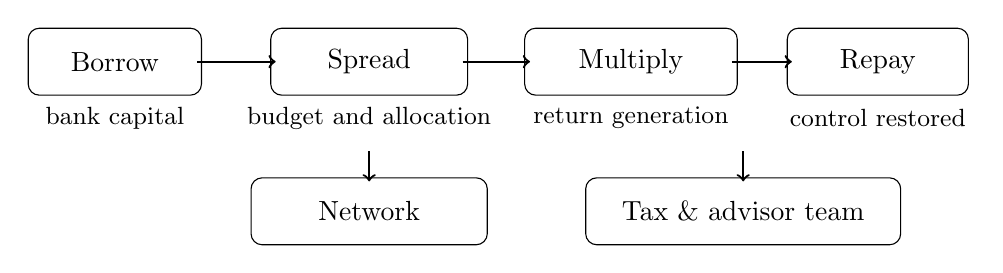
\begin{tikzpicture}[scale=0.95]
\node[draw, rounded corners, minimum width=2.2cm, minimum height=0.85cm] at (0,0) (a) {Borrow};
\node[draw, rounded corners, minimum width=2.5cm, minimum height=0.85cm] at (3.4,0) (b) {Spread};
\node[draw, rounded corners, minimum width=2.7cm, minimum height=0.85cm] at (6.9,0) (c) {Multiply};
\node[draw, rounded corners, minimum width=2.3cm, minimum height=0.85cm] at (10.2,0) (d) {Repay};

\draw[->, thick] (1.1,0) -- (2.15,0);
\draw[->, thick] (4.65,0) -- (5.55,0);
\draw[->, thick] (8.25,0) -- (9.05,0);

\node[draw, rounded corners, minimum width=3.0cm, minimum height=0.85cm] at (3.4,-2.0) (e) {Network};
\node[draw, rounded corners, minimum width=4.0cm, minimum height=0.85cm] at (8.4,-2.0) (f) {Tax \& advisor team};

\draw[->, thick] (3.4,-1.2) -- (3.4,-1.6);
\draw[->, thick] (8.4,-1.2) -- (8.4,-1.6);

\node at (0,-0.75) {\small bank capital};
\node at (3.4,-0.75) {\small budget and allocation};
\node at (6.9,-0.75) {\small return generation};
\node at (10.2,-0.75) {\small control restored};
\end{tikzpicture}
\caption{Transcript-based reconstruction of the oil case after the selling discussion. Borrowing is only the top line. Underneath it sit two deeper reserves: network, which restores motion after loss, and the technical team, which secures what has already been made.}
\end{figure}

\subsection{Question \& Answer}

\paragraph{Question.}
When does leverage help, and when is the real leverage actually the team around the money?

\paragraph{Answer.}
The lecture gives a layered answer. Borrowed money helps when it is moved rather than hoarded, when it is spread intelligently and brought back under control. But that is only the upper surface. The deeper leverage lies in the network that can restart the engine and in the advisory shell that keeps capital legally, structurally, and administratively intact. Debt may accelerate. Team and network determine durability.

At the end of the interview the host pauses for a useful recap. The point is not merely that one woman in oil made money. The point is that wealth is distributed across more industries than the naive imagination usually grants. That transition matters because the next case will again begin from an object and then surprise us by what lies underneath.

\section{The Solidcore Case: From \(\$175{,}000\) to \(\$100\) Million}

We move now to the design district and a baby-blue Bentley. The pattern at first looks familiar. The host asks what she does. She says she is an entrepreneur and investor. But the lecture becomes sharper very quickly. She sold her company in 2023. Her personal equity was worth about \(\$90\) million, and the company itself was worth a little over \(\$300\) million:
\begin{equation}
E_{\text{exit}} \approx \$90\,\text{million},
\qquad
V_{\text{company}} \gtrsim \$300\,\text{million}.
\end{equation}
The transcript briefly misfires into ``billion'' in the host's response, but the scale of the case makes clear that millions are intended.

A cautious ownership estimate is therefore
\begin{equation}
f_{\text{equity}}
\approx
\frac{E_{\text{exit}}}{V_{\text{company}}}
\approx
\frac{90}{300}
\approx
0.30,
\end{equation}
with the obvious caveat that the true fraction is likely a little lower if the company value was indeed above \(\$300\) million rather than exactly equal to it.

Then comes the chapter's clearest numerical spine. She says she put \(\$175{,}000\) into Solidcore and that it became about \(\$100\) million in ten years:
\begin{equation}
I_0=\$175{,}000,
\qquad
V_{10}\approx \$100\,\text{million}.
\end{equation}

\paragraph{Anecdote.}
This is the moment when the lecture stops being a sequence of impressive outcomes and becomes an actual capital-transformation story. We now have an initial amount, a terminal amount, and a time horizon.

\paragraph{Claim.}
Her doctrine is correspondingly explicit. Early on, if an entrepreneur really has conviction in the special sauce, the correct move may be to bet hard on oneself. Later, after the large win, the capital regime changes. She describes herself as being in wealth-preservation mode, diversified across startups, private equity, hedge funds, the stock market, and loans.

\paragraph{Mechanism.}
The transcript lets us compute two compact summaries. First the simple multiple:
\begin{align}
M
&=
\frac{V_{10}}{I_0}
=
\frac{100{,}000{,}000}{175{,}000}
\approx 571.4.
\end{align}
Then the start-end equivalent annual growth rate:
\begin{align}
r_{\text{eq}}
&=
\left(\frac{V_{10}}{I_0}\right)^{1/10}-1
\approx 0.887.
\end{align}
So the compressed story corresponds to about \(88.7\%\) annualized growth in start-end terms. We should state that carefully. This is not the literal cash-flow history of the business. It is an editorial summary of the scale of the transformation the speaker herself narrates.

\begin{figure}[h]
\centering
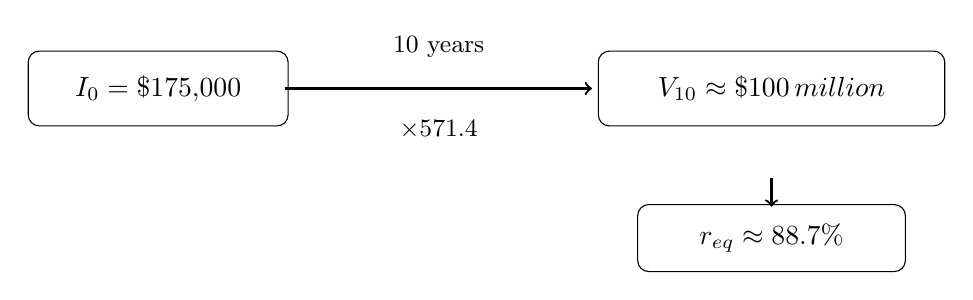
\begin{tikzpicture}[scale=0.95]
\node[draw, rounded corners, minimum width=3.3cm, minimum height=0.95cm] at (0,0) (s) {\(I_0=\$175{,}000\)};
\node[draw, rounded corners, minimum width=4.4cm, minimum height=0.95cm] at (8.2,0) (t) {\(V_{10}\approx \$100\,\text{million}\)};
\draw[->, thick] (1.7,0) -- (5.8,0);
\node at (3.75,0.55) {\small \(10\) years};
\node at (3.75,-0.55) {\small \(\times 571.4\)};
\node[draw, rounded corners, minimum width=3.4cm, minimum height=0.85cm] at (8.2,-2.0) {\(r_{\text{eq}}\approx 88.7\%\)};
\draw[->, thick] (8.2,-1.2) -- (8.2,-1.58);
\end{tikzpicture}
\caption{Transcript-based reconstruction of the Solidcore transformation. The lecture gives a start, an endpoint, and a duration, which is enough to extract both a capital multiple and a compact equivalent annual growth rate.}
\end{figure}

\subsection{Question \& Answer}

\paragraph{Question.}
When should we bet everything on ourselves, and when should we switch into preservation mode?

\paragraph{Answer.}
The lecture's answer is staged, not universal. In the entrepreneurial build phase, concentration can be rational because the founder may be the highest-conviction asset in the room. After the major win, the problem changes. The task is no longer to maximize exposure to one engine but to preserve and distribute already accumulated gains. That is why the lecture puts self-betting and diversification in sequence rather than in conflict.

\section{Critics, Customer Recognition, and the Discipline of an Easy Life}

The numerical climax naturally produces the next question: what interior arrangement made that transformation sustainable? The lecture answers by moving through criticism, customer recognition, and discipline.

\paragraph{Anecdote.}
The host asks about doubters and haters. She answers that of course they exist. But she immediately changes the frame. The people who have the most to say are very often the ones on the sidelines, in the bleachers, not actually doing the work.

\paragraph{Claim.}
This is a rule about where authority comes from. Commentary is not equal. The lecture grants more weight to builders than to spectators.

\paragraph{Mechanism.}
Her self-belief is not described as a mystical trait. It is tied to mission. She was building something that made people's lives happier and healthier, and that made her eager to continue. Purpose here is not sentimental. It is the thing that renders outside noise less binding.

The lecture then turns to Dale Carnegie and \emph{How to Win Friends and Influence People}. This shift matters. We move from ignoring the wrong voices to speaking rightly to the right people. At Solidcore, she says, they deliberately used customers' names over and over again. The operating principle is easy to write and worth keeping:
\begin{equation}
\text{name recognition}
\to
\text{felt respect}
\to
\text{return behavior}.
\end{equation}
This is one of the lecture's cleanest examples of a soft interpersonal observation turning into a retention mechanism.

The next turn is again characteristic. A life quote appears, but the lecture refuses to let it remain ornamental:
\begin{equation}
\text{easy choices} \to \text{hard life},
\qquad
\text{hard choices} \to \text{easy life}.
\end{equation}
She then grounds the aphorism in schedule:
\begin{equation}
t_{\text{wake}} \approx 5{:}30\text{--}6{:}00\ \text{a.m.},
\qquad
d_{\text{gym}} = 6/\text{week},
\end{equation}
\begin{equation}
h_{\text{volleyball}} \approx 2\text{--}3\ \text{hours/day},
\qquad
d_{\text{volleyball}} = 5/\text{week}.
\end{equation}
The implied weekly load is therefore
\begin{equation}
H_{\text{volleyball}}
=
h_{\text{volleyball}}\,d_{\text{volleyball}}
\approx
10\text{--}15\ \text{hours/week}.
\end{equation}
What matters is not the athletic detail by itself. What matters is that the lecture turns a proverb into something measurable.

\subsection{Question \& Answer}

\paragraph{Question.}
Why do hard choices feel punishing now but protective later?

\paragraph{Answer.}
Because the lecture treats discipline as intertemporal exchange. The easy act flatters the present self and weakens the future one. The hard act burdens the present self and strengthens the future one. The episode is careful here: it does not merely recite the slogan. It exhibits it through wake time, gym frequency, food discipline, volleyball hours, and the refusal to enter obviously degrading situations.

The host then asks the right follow-up question: was it worth it? Her answer is important because it prevents the chapter from becoming morally shrill. She says she did not feel as though she sacrificed anything. She loved the work, learned constantly, trusted her team, and believed the company helped people become stronger versions of themselves. Purpose changes the subjective cost of effort.

The sponsor-community interruption that follows adds no new mathematics, but it is structurally real. It breaks the rhythm, cools the intensity of the Solidcore sequence, and resets the episode before the final founder case.

\section{The Yacht-Side Beauty Founder: One Bottle, Fifteen Companies, and Strategic Differentiation}

The lecture returns to the marina. A failed approach occurs first, and the host mutters the useful persistence rule that every no is a step closer to a yes. That is a small but meaningful hinge: the host's method now begins to resemble the entrepreneurs' own doctrines.

The next interview starts, as usual, from visible wealth, but it quickly widens into time. The speaker says she is in the beauty industry, more safely normalized as the professional haircare business with worldwide reach. She has been in the beauty industry for forty-two years, and she now has fifteen companies:
\begin{equation}
t_{\text{beauty}} = 42\ \text{years},
\qquad
N_{\text{companies}} = 15.
\end{equation}
Asked for the most made in a single year, she says ``nine figures,'' which is best recorded as the lower bound
\begin{equation}
Y_{\text{hair}} \ge \$100\,\text{million}.
\end{equation}

\paragraph{Anecdote.}
The lecture immediately compresses those large numbers against a much smaller starting point. Her first business was a four-foot working square used to do hair. The transcript's unstable ``1099 and independent'' line is best understood as long-term independent-operator status rather than standard employment.

\paragraph{Claim.}
Scale, in this last case, is not a single ascent. It is a path of long duration, repeated risk, and re-creation after failure.

\paragraph{Mechanism.}
The central sequence is stark. She says she has been broke many times. The first company completely failed. Everything was lost. Then came the restart, and that restart began with one bottle because nothing else could be afforded. Ten years with a partner followed, then the partner buyout, and the endpoint is full founder ownership:
\begin{equation}
f_{\text{founder}} = 100\%.
\end{equation}
The founder trajectory can therefore be summarized as
\begin{equation}
\text{failed first company}
\to
\text{restart with one bottle}
\to
\text{buy out partner}
\to
100\% \text{ founder-owned global brand}.
\end{equation}

There is one more piece of the mechanism, and it is the right one to end on. She calls herself addicted to entrepreneurship, says she loves building, and even redefines leisure as the chance to do what she loves with people she loves while giving back. The lecture is careful not to let that drift into mere temperament. It anchors the statement in ownership history, company count, and an account of how the brand became real in the market.

\begin{figure}[h]
\centering
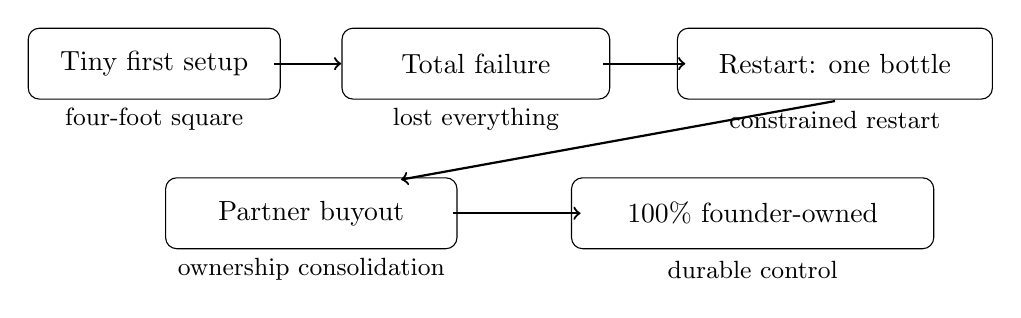
\begin{tikzpicture}[scale=0.95]
\node[draw, rounded corners, minimum width=3.2cm, minimum height=0.9cm] at (0,0) (a) {Tiny first setup};
\node[draw, rounded corners, minimum width=3.4cm, minimum height=0.9cm] at (4.3,0) (b) {Total failure};
\node[draw, rounded corners, minimum width=4.0cm, minimum height=0.9cm] at (9.1,0) (c) {Restart: one bottle};
\node[draw, rounded corners, minimum width=3.7cm, minimum height=0.9cm] at (2.1,-2.0) (d) {Partner buyout};
\node[draw, rounded corners, minimum width=4.6cm, minimum height=0.9cm] at (8.0,-2.0) (e) {\(100\%\) founder-owned};

\draw[->, thick] (1.6,0) -- (2.5,0);
\draw[->, thick] (6.0,0) -- (7.1,0);
\draw[->, thick] (9.1,-0.5) -- (3.3,-1.55);
\draw[->, thick] (4.0,-2.0) -- (5.7,-2.0);

\node at (0,-0.75) {\small four-foot square};
\node at (4.3,-0.75) {\small lost everything};
\node at (9.1,-0.75) {\small constrained restart};
\node at (2.1,-2.75) {\small ownership consolidation};
\node at (8.0,-2.75) {\small durable control};
\end{tikzpicture}
\caption{Transcript-based reconstruction of the final founder path. The lecture ends not with a single formula for becoming rich, but with a sequence: tiny start, failure, constrained restart, ownership consolidation, and durable control.}
\end{figure}

\subsection{Question \& Answer}

\paragraph{Question.}
How do we know that a brand has crossed from founder hope into real market pull?

\paragraph{Answer.}
The lecture answers through the airport story. She walks into a salon, asks whether they carry her product, and finds that they have just sold the last bottle. They are carrying it even though another brand is supposed to dominate the space. That is the test. A brand has become real when the demand exists independently of the founder's own speech, when shelf pressure appears, and when the customer speaks about the product as though it already belongs to her life.

The final advice is therefore strategic rather than merely motivational. It is not what one has, but what one does with what one has. It is not even only a matter of working harder rather than smarter. The sharper word is strategy:
\begin{equation}
\text{crowded path} \to \text{differentiation},
\qquad
\text{zig when they zag}.
\end{equation}
That is the lecture's last compression. Exceptional outcomes are not presented as a reward for generic effort alone. They are presented as the result of off-angle movement in a crowded field.

\section{Summary}

The lecture begins by scattering glamorous fragments and ends by ordering them into mechanisms. First we are shown yachts, exits, expensive objects, and the word ``billionaire.'' Then the chapter slowly assigns those surfaces to deeper structures: years in business, the six-to-seven-million-dollar oil range, a \(\$28\) million deal, borrowing and spreading capital, a ten-phone-call network reserve, a tax-and-advisor shell, a founder's \(\$90\) million exit against a company worth a little over \(\$300\) million, the transformation
\[
\$175{,}000 \to \$100\,\text{million in 10 years},
\]
a customer-retention rule built from names and respect, a discipline schedule that makes the hard-choice aphorism measurable, and finally a forty-two-year founder trajectory built through failure, restart, buyout, and full ownership. What the lecture teaches, taken seriously, is that wealth is not explained by the object in front of us. It is explained by the sequence underneath it.